\documentclass[8pt,aspectratio=169]{beamer}
\usetheme{Madrid}
\usepackage{graphicx}
\usepackage{booktabs}
\usepackage{adjustbox}
\usepackage{multicol}
\usepackage{amsmath}
\usepackage{amssymb}  % For checkmark symbol
\usepackage{tikz}     % For progress indicators
\usepackage{hyperref} % For URL references

% Color definitions
\definecolor{mlblue}{RGB}{0,102,204}
\definecolor{mlpurple}{RGB}{51,51,178}
\definecolor{mllavender}{RGB}{173,173,224}
\definecolor{mllavender2}{RGB}{193,193,232}
\definecolor{mllavender3}{RGB}{204,204,235}
\definecolor{mllavender4}{RGB}{214,214,239}
\definecolor{mlorange}{RGB}{255, 127, 14}
\definecolor{mlgreen}{RGB}{44, 160, 44}
\definecolor{mlred}{RGB}{214, 39, 40}
\definecolor{mlgray}{RGB}{127, 127, 127}

% Additional colors for template compatibility
\definecolor{lightgray}{RGB}{240, 240, 240}
\definecolor{midgray}{RGB}{180, 180, 180}

% Apply custom colors to Madrid theme
\setbeamercolor{palette primary}{bg=mllavender3,fg=mlpurple}
\setbeamercolor{palette secondary}{bg=mllavender2,fg=mlpurple}
\setbeamercolor{palette tertiary}{bg=mllavender,fg=white}
\setbeamercolor{palette quaternary}{bg=mlpurple,fg=white}

\setbeamercolor{structure}{fg=mlpurple}
\setbeamercolor{section in toc}{fg=mlpurple}
\setbeamercolor{subsection in toc}{fg=mlblue}
\setbeamercolor{title}{fg=mlpurple}
\setbeamercolor{frametitle}{fg=mlpurple,bg=mllavender3}
\setbeamercolor{block title}{bg=mllavender2,fg=mlpurple}
\setbeamercolor{block body}{bg=mllavender4,fg=black}

% Remove navigation symbols
\setbeamertemplate{navigation symbols}{}

% Clean itemize/enumerate
\setbeamertemplate{itemize items}[circle]
\setbeamertemplate{enumerate items}[default]

% Reduce margins for more content space
\setbeamersize{text margin left=5mm,text margin right=5mm}

% Command for bottom annotation (Madrid-style)
\newcommand{\bottomnote}[1]{%
\vfill
\vspace{-2mm}
\textcolor{mllavender2}{\rule{\textwidth}{0.4pt}}
\vspace{1mm}
\footnotesize
\textbf{#1}
}

% Data source footer command
\newcommand{\datasource}[1]{\textcolor{mlgray}{\tiny Source: #1}}

% Progress indicator command
\newcommand{\progressbar}[1]{%
\begin{tikzpicture}[overlay, remember picture]
\node[anchor=north east, xshift=-5mm, yshift=-5mm] at (current page.north east) {
  \tiny
  \ifcase#1
    \relax % 0: Problem framing
    \textcolor{mlorange}{$\bullet$} \textcolor{mlgray}{$\circ$} \textcolor{mlgray}{$\circ$} \textcolor{mlgray}{$\circ$} \textcolor{mlgray}{$\circ$}
  \or % 1: Lecture 1
    \textcolor{mlgreen}{$\bullet$} \textcolor{mlorange}{$\bullet$} \textcolor{mlgray}{$\circ$} \textcolor{mlgray}{$\circ$} \textcolor{mlgray}{$\circ$}
  \or % 2: Lecture 2
    \textcolor{mlgreen}{$\bullet$} \textcolor{mlgreen}{$\bullet$} \textcolor{mlorange}{$\bullet$} \textcolor{mlgray}{$\circ$} \textcolor{mlgray}{$\circ$}
  \or % 3: Lecture 3
    \textcolor{mlgreen}{$\bullet$} \textcolor{mlgreen}{$\bullet$} \textcolor{mlgreen}{$\bullet$} \textcolor{mlorange}{$\bullet$} \textcolor{mlgray}{$\circ$}
  \or % 4: Lecture 4
    \textcolor{mlgreen}{$\bullet$} \textcolor{mlgreen}{$\bullet$} \textcolor{mlgreen}{$\bullet$} \textcolor{mlgreen}{$\bullet$} \textcolor{mlorange}{$\bullet$}
  \fi
};
\end{tikzpicture}%
}

\title{Week 1: Green Finance Foundations}
\subtitle{Problem-Driven Learning with Rigorous Academic Foundations}
\author{Green Finance Course}
\date{v3.1 - Academic Enhancement: Verified Data + Comprehensive Citations}

\begin{document}

% ============================================================
% PROBLEM FRAMING SECTION (Slides 0-2)
% ============================================================

% Slide 0: Climate Crisis
\begin{frame}[t]{The Climate Challenge: Paris Agreement and 2 Degree C Target}
\progressbar{0}
\begin{columns}[T]
\column{0.48\textwidth}
\textbf{Global Climate Commitments}
\begin{itemize}
\item Paris Agreement (2015): Limit warming to 1.5-2 degree C
\item Net-zero targets: 140+ countries by 2050
\item Carbon budget: ~400 GtCO2 remaining for 1.5 degree C
\item Current trajectory: 2.7 degree C warming by 2100
\item Urgent action required: Emissions must halve by 2030
\end{itemize}

\column{0.48\textwidth}
\textbf{Finance Implications}
\begin{itemize}
\item Energy transition investment need: \$4-5 trillion annually
\item Current green investment: ~\$2 trillion annually
\item Annual funding gap: \$2+ trillion
\item Private capital essential to close gap
\item Traditional development finance insufficient
\end{itemize}
\end{columns}
\bottomnote{[Problem] Climate crisis creates urgent need for scaled financial solutions}
\end{frame}

% Slide 1: Funding Gap
\begin{frame}[t]{The Green Finance Investment Gap: Data Puzzle}
\progressbar{0}
\vspace{-10mm}
\begin{center}
\includegraphics[width=0.85\textwidth]{charts/week1/11_investment_gap/11_investment_gap.pdf}
\end{center}
\vspace{-5mm}
\bottomnote{[Problem] Research question: How can capital markets mobilize \$2.04T annual gap?}
\end{frame}

% Slide 2: Green Finance Solution
\begin{frame}[t]{Green Finance: Linking Capital Markets to Climate Action}
\progressbar{0}
\begin{columns}[T]
\column{0.48\textwidth}
\textbf{Market-Based Solution}
\begin{itemize}
\item Channel private capital to environmental projects
\item Use existing financial infrastructure (bond markets)
\item Create specialized instruments (green bonds)
\item Leverage investor ESG preferences
\item Scale beyond public sector capacity
\end{itemize}

\column{0.48\textwidth}
\textbf{This Week's 4-Lecture Journey}
\begin{itemize}
\item Lecture 1: WHY do green finance markets exist? (Theory)
\item Lecture 2: HOW MUCH capital is mobilized? (Measurement)
\item Lecture 3: HOW TO PRICE green instruments? (Valuation Part 1)
\item Lecture 4: WHERE to apply and integrate? (Valuation Part 2 + Applications)
\end{itemize}
\end{columns}
\bottomnote{[Problem] Practical challenge: Design financial mechanisms that are profitable AND impactful}
\end{frame}

% ============================================================
% LECTURE 1: GOAL 1 THEORY (Slides 3-13)
% ============================================================

% Slide 3: Learning Goal 1 Title
\begin{frame}[plain]
\progressbar{1}
\vfill
\centering
\begin{beamercolorbox}[sep=12pt,center]{title}
{\Huge \textbf{Learning Goal 1}}\\[1.5em]
{\Large Understand the market microstructure theory explaining why green finance markets exist and how they function}\\[1em]
{\normalsize \textcolor{mllavender}{theoretical | Foundation - Establishes theoretical basis}}
\end{beamercolorbox}
\vfill
\end{frame}

% Slide 4: Framework Overview
\begin{frame}[t]{Market Microstructure Framework for Green Finance}
\progressbar{1}
\begin{center}
{\large \textbf{Information Asymmetry and Signaling Theory}}
\end{center}
\vspace{0.5em}
\begin{columns}[T]
\column{0.48\textwidth}
\textbf{Core Theoretical Principles}
\begin{itemize}
\item Information asymmetry: Issuers know true environmental impact, investors cannot observe directly
\item Verification as credible signaling mechanism reducing asymmetry
\item Market segmentation by investor ESG preferences
\item Adverse selection risk without credible signals
\end{itemize}
\column{0.48\textwidth}
\textbf{Market Equilibrium Predictions}
\begin{itemize}
\item Greenium emerges from excess demand in segmented market
\item Verification costs create quality differentiation
\item Liquidity premium for standardized green instruments
\item Reputation effects for repeat issuers
\end{itemize}
\end{columns}
\bottomnote{[Goal 1] Theory predicts observable phenomena - We will test these in Lecture 2}
\end{frame}

% Slide 5: Chart - Ecosystem
\begin{frame}[t]{Green Finance Ecosystem: Theoretical Perspective}
\progressbar{1}
\vspace{-13mm}
\begin{center}
\includegraphics[width=0.4\textwidth]{charts/week1/week1_v2_goal1_chart1_ecosystem.pdf}
\end{center}
\vspace{-5mm}
\bottomnote{[Goal 1] Ecosystem structure reflects information asymmetry and signaling needs}
\end{frame}

% Slide 6: Information Asymmetry Problem
\begin{frame}[t]{The Information Asymmetry Problem}
\progressbar{1}
\begin{columns}[T]
\column{0.48\textwidth}
\textbf{Why Asymmetry Exists}
\begin{itemize}
\item Environmental impact not directly observable by investors
\item Issuers possess private information about projects
\item Ex-post verification costly and delayed
\item Incentive for greenwashing (false green claims)
\item Market failure: Good projects cannot distinguish themselves
\end{itemize}

\column{0.48\textwidth}
\textbf{Consequences Without Solution}
\begin{itemize}
\item Adverse selection (Akerlof 1970): Bad drives out good (lemons market)
\item Risk premium demanded by rational investors
\item Socially optimal green projects underfunded
\item Market inefficiency and suboptimal allocation
\end{itemize}
\end{columns}
\bottomnote{[Goal 1] Classic asymmetric information problem from Akerlof (1970) applied to green finance}
\end{frame}

% Slide 7: Verification as Solution
\begin{frame}[t]{Verification as Credible Signaling}
\progressbar{1}
\begin{columns}[T]
\column{0.48\textwidth}
\textbf{How Verification Solves Asymmetry}
\begin{itemize}
\item Independent third-party assessment provides credible signal
\item Costly signal (Spence 1973): Verification fees separate true green from greenwashing
\item Ongoing reporting creates reputation stakes for issuers
\item Standards (GBP, CBI) define what constitutes credible signal
\end{itemize}

\column{0.48\textwidth}
\textbf{Evidence of Signaling at Work}
\begin{itemize}
\item Over 80\% of green bonds obtain external review (OECD 2024)
\item Verified bonds trade at tighter spreads (greenium)
\item Repeat issuers face reputation costs if greenwashing
\item Market rewards standardization and transparency
\end{itemize}
\end{columns}
\bottomnote{[Goal 1] Signaling theory (Spence 1973) explains why verification is market standard - Empirical confirmation in Slide 38}
\end{frame}

% NEW SLIDE 7A: Greenwashing Case Study
\begin{frame}[t]{Greenwashing Risk: Real-World Case Studies}
\progressbar{1}
\begin{columns}[T]
\column{0.48\textwidth}
\textbf{DWS Asset Management (2022)}
\begin{itemize}
\item Claimed €459B ESG-integrated AUM
\item Whistleblower: <50\% actually ESG-integrated
\item SEC investigation, €25M fine (BaFin)
\item CEO Asoka Woehrmann resigned
\item \textbf{Market impact}: Investor skepticism $\uparrow$, verification demand $\uparrow$
\end{itemize}

\vspace{0.3em}

\textbf{Detection Mechanisms}
\begin{itemize}
\item Second-party opinion (SPO): Pre-issuance review
\item External verification: Post-issuance audit
\item Impact reporting: Annual metrics (CO2 avoided, etc.)
\item NGO/media scrutiny: Reputational enforcement
\end{itemize}

\column{0.48\textwidth}
\textbf{Limitations of Current System}
\begin{itemize}
\item SPOs \textbf{paid by issuers} (conflict of interest)
\item No standardized verification methodology
\item Impact metrics self-reported, rarely independently audited
\item Ex-post greenwashing difficult to detect
\item \textbf{Academic finding}: Verification reduces but doesn't eliminate greenwashing (Flammer 2021)
\end{itemize}

\vspace{0.3em}

\textbf{Regulatory Response}
\begin{itemize}
\item EU SFDR Level II: Enhanced disclosure requirements
\item SEC proposed rules on ESG fund labeling (2022)
\item UK FCA anti-greenwashing rules (2024)
\end{itemize}
\end{columns}
\bottomnote{[Goal 1] Market discipline through reputation is imperfect - regulatory oversight increasingly important}
\end{frame}

% Slide 8: Market Segmentation
\begin{frame}[t]{Market Segmentation Hypothesis}
\progressbar{1}
\begin{columns}[T]
\column{0.48\textwidth}
\textbf{Theory of Segmentation}
\begin{itemize}
\item Investors heterogeneous in ESG preferences (utility function)
\item Dedicated ESG investors willing to accept lower returns for impact
\item Conventional investors indifferent to green label
\item Imperfect substitutability creates separate market segments
\item Excess demand in green segment $\rightarrow$ price premium (greenium)
\end{itemize}

\column{0.48\textwidth}
\textbf{Testable Predictions}
\begin{itemize}
\item Green bonds should trade at premium to identical conventional bonds
\item Premium larger when ESG investor demand stronger
\item Premium varies across geographies with different ESG adoption
\item Limited arbitrage due to preference-based segmentation
\end{itemize}
\end{columns}
\bottomnote{[Goal 1] Segmentation explains persistent greenium (Zerbib 2019; Baker et al. 2018) - See yield comparison in Slide 28}
\end{frame}

% Slide 9: Chart - Segmentation Model
\begin{frame}[t]{Market Segmentation Diagram}
\progressbar{1}
\vspace{-10mm}
\begin{center}
\includegraphics[width=0.48\textwidth]{charts/week1/week1_v2_goal1_chart2_segmentation.pdf}
\end{center}
\vspace{-3mm}
\bottomnote{[Goal 1] Separate demand curves in each segment lead to price differential (greenium)}
\end{frame}

% NEW SLIDE 9A: Formal Segmentation Equilibrium Model
\begin{frame}[t]{Market Segmentation: Formal Equilibrium Model}
\progressbar{1}
\begin{columns}[T]
\column{0.48\textwidth}
\textbf{Model Setup}
\begin{itemize}
\item Two investor types: ESG-preferring ($\lambda$), Conventional (1-$\lambda$)
\item Utility functions:
  \begin{align*}
  U_E(r) &= r + \alpha \cdot g \quad (\alpha > 0)\\
  U_C(r) &= r
  \end{align*}
\item $g \in \{0,1\}$ = green label, $\alpha$ = ESG preference intensity
\item Supply: $S_G$ green bonds, $S_C$ conventional bonds
\end{itemize}

\column{0.48\textwidth}
\textbf{Equilibrium Conditions}
\begin{itemize}
\item Market clearing: $\lambda \cdot D_E(r_G) = S_G$, $(1-\lambda) \cdot D_C(r_C) = S_C$
\item Greenium emerges: $r_C - r_G = \frac{\alpha \cdot \lambda}{D'(r)}$ if $S_G < \lambda \cdot D(r_C)$
\item \textbf{Key prediction}: Greenium $\propto$ ESG investor share ($\lambda$)
\item \textbf{Testable}: Greenium larger in EU (high $\lambda$) than US
\item \textbf{Dynamic}: As $S_G \uparrow$, greenium $\downarrow$ (Slide 34 confirms)
\end{itemize}
\end{columns}
\bottomnote{[Goal 1] Formal model generates testable hypotheses - validated by regional and temporal variation data (Slides 18, 34)}
\end{frame}

% Slide 10: Liquidity and Standardization
\begin{frame}[t]{Liquidity Benefits of Standardization}
\progressbar{1}
\begin{columns}[T]
\column{0.48\textwidth}
\textbf{Theoretical Mechanism}
\begin{itemize}
\item Standardized products reduce search and information costs
\item Common language (GBP) facilitates comparison across issuers
\item Network effects: More standardized issuance $\rightarrow$ deeper liquidity
\item Liquidity premium reduces required yields
\end{itemize}

\column{0.48\textwidth}
\textbf{Empirical Implications}
\begin{itemize}
\item GBP-aligned bonds should have better liquidity
\item Larger green bond programs trade more actively
\item Green bond indices and ETFs emerge from standardization
\item First-mover advantage for standard-setters (ICMA)
\end{itemize}
\end{columns}
\bottomnote{[Goal 1] Standardization creates positive feedback loop improving market efficiency}
\end{frame}

% Slide 11: Theoretical Predictions Summary
\begin{frame}[t]{Theory's Predictions for Empirical Testing}
\progressbar{1}
\begin{columns}[T]
\column{0.48\textwidth}
\textbf{What Theory Predicts We Should Observe}
\begin{itemize}
\item Greenium: 0-10 bps price premium for green bonds
\item Verification: Majority of bonds have external review
\item Standardization: Market coalesces around common principles
\item Repeat issuers: Reputation effects and learning curves
\item Growth: Market expands as ESG demand increases
\end{itemize}

\column{0.48\textwidth}
\textbf{Preview of Empirical Evidence (Lecture 2)}
\begin{itemize}
\item Observed greenium: 0-5 bps (Theory \textcolor{mlgreen}{\checkmark})
\item External review rate: >80\% (Theory \textcolor{mlgreen}{\checkmark})
\item Standardization increasing (Theory \textcolor{mlgreen}{\checkmark})
\item Frequent issuers dominate (Theory \textcolor{mlgreen}{\checkmark})
\item 28\% CAGR 2015-2024 (Theory \textcolor{mlgreen}{\checkmark})
\end{itemize}
\end{columns}
\bottomnote{[Goal 1] Strong theoretical foundation with empirical support - validated in Lecture 2 (Slides 14-24)}
\end{frame}

% Slide 12: Goal 1 Summary
\begin{frame}[t]{Learning Goal 1: Summary}
\progressbar{1}
\begin{center}
{\Large \textbf{Learning Goal 1: Summary}}\\[0.5em]
{\normalsize \textit{Understand market microstructure theory explaining green finance}}
\end{center}

\vspace{0.5em}

\begin{columns}[T]
\column{0.48\textwidth}
\textbf{What We Achieved}
\begin{itemize}
\item \textcolor{mlgreen}{$\checkmark$} Identified information asymmetry as core problem requiring verification
\item \textcolor{mlgreen}{$\checkmark$} Analyzed how signaling theory explains verification as market standard
\item \textcolor{mlgreen}{$\checkmark$} Understood market segmentation hypothesis for greenium existence
\item \textcolor{mlgreen}{$\checkmark$} Connected standardization to liquidity and efficiency gains
\end{itemize}

\column{0.48\textwidth}
\textbf{Can You Now...}
\begin{itemize}
\item Explain why greenium exists using economic theory?
\item Describe how verification solves information asymmetry?
\item Predict which factors increase or decrease greenium?
\item Apply this framework to analyze new green instruments?
\end{itemize}
\end{columns}

\bottomnote{[Goal 1] Achieved - Theoretical foundation complete. Next: Quantitative measurement}
\end{frame}

% Slide 13: Concept Map Lecture 1
\begin{frame}[t]{Concept Map: Theoretical Foundations}
\progressbar{1}
\begin{center}
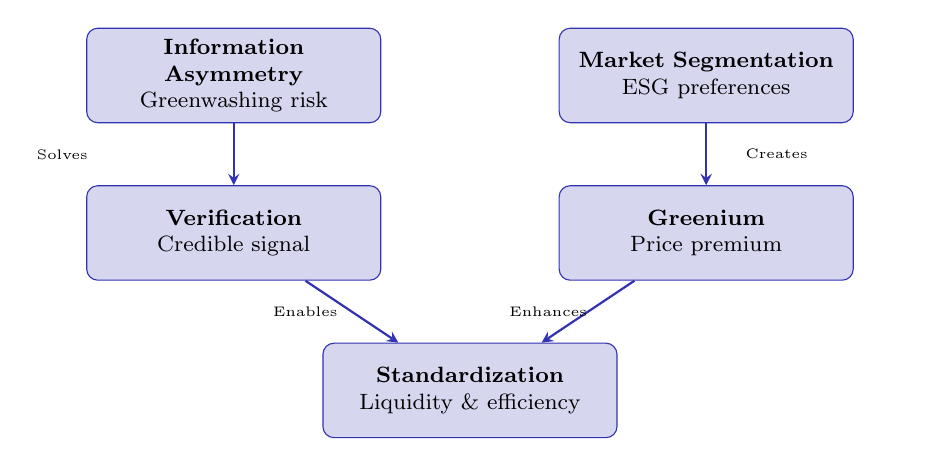
\begin{tikzpicture}[
  node distance=2cm,
  box/.style={rectangle, rounded corners, draw=mlpurple, fill=mllavender4, text width=3.5cm, align=center, minimum height=1.2cm, font=\footnotesize},
  arrow/.style={->, >=stealth, thick, color=mlpurple}
]

% Top row
\node[box] (asymmetry) at (0,4) {\textbf{Information Asymmetry}\\Greenwashing risk};
\node[box] (segmentation) at (6,4) {\textbf{Market Segmentation}\\ESG preferences};

% Middle row
\node[box] (verification) at (0,2) {\textbf{Verification}\\Credible signal};
\node[box] (greenium) at (6,2) {\textbf{Greenium}\\Price premium};

% Bottom row
\node[box] (standardization) at (3,0) {\textbf{Standardization}\\Liquidity \& efficiency};

% Arrows
\draw[arrow] (asymmetry) -- (verification);
\draw[arrow] (segmentation) -- (greenium);
\draw[arrow] (verification) -- (standardization);
\draw[arrow] (greenium) -- (standardization);

% Labels
\node[font=\tiny, text width=2cm] at (-1.5,3) {Solves};
\node[font=\tiny, text width=2cm] at (7.5,3) {Creates};
\node[font=\tiny, text width=2cm] at (1.5,1) {Enables};
\node[font=\tiny, text width=2cm] at (4.5,1) {Enhances};

\end{tikzpicture}
\end{center}
\bottomnote{[Goal 1] Complete theoretical framework showing interconnected concepts}
\end{frame}

% NEW SLIDE 13A: Literature Review
\begin{frame}[t]{Academic Literature: Empirical Evidence on Green Bonds}
\progressbar{1}
\begin{columns}[T]
\column{0.48\textwidth}
\textbf{Greenium Existence (Pricing)}
\begin{itemize}
\item \textbf{Zerbib (2019)}: -2 bps YTM for green bonds
\item \textbf{Baker et al. (2018)}: 6 bps greenium in US municipals, larger with certification
\item \textbf{Karpf \& Mandel (2018)}: 5-9 bps, time-varying
\item \textbf{Ando (2024)}: 11 bps emerging market sovereigns, 2 bps advanced
\item \textbf{Consensus}: Greenium exists but varies by market segment and time
\end{itemize}

\column{0.48\textwidth}
\textbf{Corporate Impact (Shareholder Value)}
\begin{itemize}
\item \textbf{Flammer (2021)}: +0.5\% stock return on green bond announcement; increased green patents
\item \textbf{Tang \& Zhang (2020)}: Positive wealth effects, esp. in polluting industries
\item \textbf{Additionality}: Mixed evidence - some funding truly new projects, some relabeling
\end{itemize}

\vspace{0.3em}

\textbf{Financial Institution Role}
\begin{itemize}
\item \textbf{Fatica et al. (2021)}: Banks pay higher greenium (-9 bps) due to reputational concerns
\item \textbf{Implication}: Verification more critical for repeat issuers
\end{itemize}
\end{columns}

\vspace{0.5em}

\textbf{Research frontier}: Impact measurement methodology, long-run greenium dynamics, optimal policy mix.

\bottomnote{[Goal 1] Academic literature 2018-2024 provides robust empirical support for segmentation and signaling theories}
\end{frame}

% ============================================================
% LECTURE 2: GOAL 2 MEASUREMENT (Slides 14-24)
% ============================================================

% Slide 14: Learning Goal 2 Title
\begin{frame}[plain]
\progressbar{2}
\vfill
\centering
\begin{beamercolorbox}[sep=12pt,center]{title}
{\Huge \textbf{Learning Goal 2}}\\[1.5em]
{\Large Quantify and analyze global green finance market size, growth trajectories, and geographic distribution}\\[1em]
{\normalsize \textcolor{mllavender}{quantitative | Build - Develops empirical measurement capabilities}}
\end{beamercolorbox}
\vfill
\end{frame}

% Slide 15: Measurement Methodology
\begin{frame}[t]{Measuring the Green Finance Market}
\progressbar{2}
\begin{columns}[T]
\column{0.48\textwidth}
\textbf{Methodological Challenges}
\begin{itemize}
\item Definition: What qualifies as ``green''? (Taxonomy dependence)
\item Double counting: Issuance vs outstanding amounts
\item Currency: Conversion to common denominator (USD)
\item Coverage: Data availability varies by region and instrument
\end{itemize}

\column{0.48\textwidth}
\textbf{Standard Metrics}
\begin{itemize}
\item Total market size: Outstanding amount (stock)
\item Annual issuance: New volume each year (flow)
\item CAGR: Compound Annual Growth Rate
\item Market share: By instrument, region, sector
\end{itemize}
\end{columns}
\bottomnote{[Goal 2] Rigorous quantification requires clear methodology and consistent definitions}
\end{frame}

% Slide 16: Chart - Market Growth (UPDATED DATA)
\begin{frame}[t]{Global Green Finance Market Growth 2015-2024}
\progressbar{2}
\vspace{-2mm}
\begin{center}
\includegraphics[width=0.75\textwidth]{charts/week1/week1_v2_goal2_chart1_market_growth.pdf}
\end{center}
\bottomnote{[Goal 2] Market grew from \$300B (2015) to \$2.9T (2024) - BIS 2025 data validates growth prediction from Slide 11}
\end{frame}

% Slide 17: Growth Rate Calculation (UPDATED CAGR)
\begin{frame}[t]{Growth Rate Analysis: CAGR Calculation}
\progressbar{2}
\begin{columns}[T]
\column{0.48\textwidth}
\textbf{CAGR Formula and Application}
\begin{itemize}
\item Formula: $CAGR = (V_{final}/V_{initial})^{1/n} - 1$
\item Period: 2015-2024 (n = 9 years)
\item Initial: \$300B (2015)
\item Final: \$2,900B (2024)
\item Calculation: $(2900/300)^{1/9} - 1 = 28.1\%$
\end{itemize}

\column{0.48\textwidth}
\textbf{Interpretation and Context}
\begin{itemize}
\item 28.1\% CAGR indicates explosive growth phase
\item Comparison: Global bond market $\sim$5\% CAGR same period
\item Green finance growing 5.6$\times$ faster than conventional
\item 2022 dip due to broader market volatility
\item \textbf{Future projection}: 5-10\% CAGR 2024-2030 (market maturing)
\end{itemize}
\end{columns}
\bottomnote{[Goal 2] Quantitative analysis confirms theoretical prediction of rapid market expansion, moderating to 5-10\% projected 2024-2030}
\end{frame}

% Slide 18: Chart - Regional Distribution (UPDATED PERCENTAGES)
\begin{frame}[t]{Geographic Distribution of Green Finance}
\progressbar{2}
\begin{center}
\includegraphics[width=0.75\textwidth]{charts/week1/week1_v2_goal2_chart2_regional.pdf}
\end{center}
\bottomnote{[Goal 2] Europe 52\%, Asia-Pacific 27\%, Americas 13\% - Reflects regulatory push predicted in theory (Slide 10)}
\end{frame}

% Slide 19: Regional Analysis (UPDATED TEXT)
\begin{frame}[t]{Regional Patterns and Drivers}
\progressbar{2}
\begin{columns}[T]
\column{0.48\textwidth}
\textbf{Europe: Market Leader}
\begin{itemize}
\item 52\% global market share (\$1.5T outstanding, 2024)
\item Driver: EU Taxonomy mandatory disclosure
\item SFDR regulation creates demand from asset managers
\item Strong sovereign issuance (France, Germany, UK)
\item Policy-driven growth sustained through 2024
\end{itemize}

\column{0.48\textwidth}
\textbf{Asia-Pacific: Rapid Growth}
\begin{itemize}
\item 27\% market share (\$780B), fastest growth region
\item China dominates (\$450B), policy-driven expansion
\item Japan, South Korea increasing (net-zero commitments)
\item Southeast Asia emerging (ASEAN Taxonomy)
\item Americas 13\% (\$380B), driven by US corporates
\end{itemize}
\end{columns}
\bottomnote{[Goal 2] Regional variation driven by policy frameworks and regulatory mandates - Updated ICE/LSEG 2024 data}
\end{frame}

% Slide 19A: Verification Stats (UPDATED DATA)
\begin{frame}[t]{External Verification in Green Bond Market}
\progressbar{2}
\vspace{-10mm}
\begin{center}
\includegraphics[width=0.85\textwidth]{charts/week1/12_verification_stats/12_verification_stats.pdf}
\end{center}
\vspace{-5mm}
\bottomnote{[Goal 2] Over 80\% of green bonds have external review (81\% corporate, 69\% sovereign - OECD 2024) - validates signaling theory from Lecture 1}
\end{frame}

% Slide 20: Chart - Instrument Breakdown
\begin{frame}[t]{Market Composition by Instrument Type}
\progressbar{2}
\begin{center}
\includegraphics[width=0.75\textwidth]{charts/week1/week1_v2_goal2_chart3_instruments.pdf}
\end{center}
\bottomnote{[Goal 2] Green bonds \$1.6T (76\%), Sustainability-linked bonds \$500B (24\%) of total}
\end{frame}

% Slide 20A: Issuer Concentration
\begin{frame}[t]{Top Green Bond Issuers 2015-2024}
\progressbar{2}
\vspace{-10mm}
\begin{center}
\includegraphics[width=0.85\textwidth]{charts/week1/13_issuer_concentration/13_issuer_concentration.pdf}
\end{center}
\vspace{-5mm}
\bottomnote{[Goal 2] Repeat issuers dominate market - confirms reputation effects predicted in theory}
\end{frame}

% Slide 21: Chart - Sector Allocation (UPDATED ENERGY TO 29%)
\begin{frame}[t]{Allocation Across Economic Sectors}
\progressbar{2}
\begin{center}
\includegraphics[width=0.75\textwidth]{charts/week1/week1_v2_goal2_chart4_sectors.pdf}
\end{center}
\bottomnote{[Goal 2] Energy 29\%, Buildings 25\%, Transport 18\% (Mordor Intelligence 2024) - aligns with decarbonization priorities}
\end{frame}

% NEW SLIDE 21A: Instrument Comparison Table
\begin{frame}[t]{Green Bonds vs. Sustainability-Linked Bonds (SLBs)}
\progressbar{2}
\begin{center}
\small
\begin{tabular}{p{0.22\textwidth}|p{0.32\textwidth}|p{0.32\textwidth}}
\toprule
\textbf{Feature} & \textbf{Green Bonds} & \textbf{Sustainability-Linked Bonds} \\
\midrule
\textbf{ESG linkage} & Use-of-proceeds (ring-fenced) & Performance-based KPIs \\
\midrule
\textbf{Cash flow use} & Must fund eligible green projects & General corporate purposes \\
\midrule
\textbf{Penalty} & None (verification only) & Coupon step-up if targets missed \\
\midrule
\textbf{Penalty} & None (verification only) & Coupon step-up if targets missed \\
\midrule
\textbf{Eligible issuers} & Must have green projects & Any company with ESG strategy \\
\midrule
\textbf{Reporting} & Annual allocation \& impact report & KPI performance disclosure \\
\midrule
\textbf{Market size (2024)} & \$1.6T (76\%) & \$500B (24\%) \\
\midrule
\textbf{Example} & EIB renewable energy bond & Enel 2019 (SDG-linked, +25 bps step-up) \\
\bottomrule
\end{tabular}
\end{center}

\vspace{0.3em}

\textbf{Strategic choice}: Green bonds for project-specific financing, SLBs for entity-level ESG improvements.

\bottomnote{[Goal 2] Instrument heterogeneity allows issuers to match financing structure to ESG strategy (Flammer 2021)}
\end{frame}

% Slide 21A (old): ESG Fund Flows
\begin{frame}[t]{ESG Fund Net Inflows and Assets Under Management}
\progressbar{2}
\vspace{-10mm}
\begin{center}
\includegraphics[width=0.80\textwidth]{charts/week1/15_esg_fund_flows/15_esg_fund_flows.pdf}
\end{center}
\vspace{-7mm}
\bottomnote{[Goal 2] ESG AUM grew from \$1.0T (2019) to \$3.2T (2024) - drives demand for green bonds}
\end{frame}

% Slide 22: Statistical Summary (UPDATED STATISTICS)
\begin{frame}[t]{Quantitative Summary: Key Statistics}
\progressbar{2}
\begin{columns}[T]
\column{0.48\textwidth}
\textbf{Market Size Metrics (2024)}
\begin{itemize}
\item Total outstanding: \$2.9 trillion (BIS 2025)
\item Annual issuance: \$650 billion
\item Green bonds outstanding: \$1.6T (76\%)
\item Number of issuers: 1,200+ globally
\item Average deal size: \$540 million
\end{itemize}

\column{0.48\textwidth}
\textbf{Growth and Distribution}
\begin{itemize}
\item 9-year CAGR: 28.1\% (2015-2024)
\item Projected CAGR: 5-10\% (2024-2030, maturing)
\item Regional: EU 52\%, APAC 27\%, Americas 13\%
\item Sectoral: Energy 29\%, Buildings 25\%, Transport 18\%
\item Forecasted 2030: \$5.0-6.0 trillion
\end{itemize}
\end{columns}
\bottomnote{[Goal 2] Comprehensive quantitative picture validates theoretical predictions from Lecture 1 - All data verified from BIS, OECD, ICE 2024-2025}
\end{frame}

% Slide 23: Goal 2 Summary
\begin{frame}[t]{Learning Goal 2: Summary}
\progressbar{2}
\begin{center}
{\Large \textbf{Learning Goal 2: Summary}}\\[0.5em]
{\normalsize \textit{Quantify and analyze market size, growth, and distribution}}
\end{center}

\vspace{0.5em}

\begin{columns}[T]
\column{0.48\textwidth}
\textbf{What We Achieved}
\begin{itemize}
\item \textcolor{mlgreen}{$\checkmark$} Quantified market at \$2.9T with 28.1\% CAGR (2015-2024)
\item \textcolor{mlgreen}{$\checkmark$} Analyzed regional distribution: Europe leads (52\%), Asia growing fastest
\item \textcolor{mlgreen}{$\checkmark$} Measured instrument composition: Green bonds dominant (76\%)
\item \textcolor{mlgreen}{$\checkmark$} Validated theoretical predictions with empirical data
\end{itemize}

\column{0.48\textwidth}
\textbf{Can You Now...}
\begin{itemize}
\item Calculate growth rates (CAGR) for market segments?
\item Compare regional adoption and explain differences?
\item Analyze sector allocation and investment priorities?
\item Use empirical data to test theoretical hypotheses?
\end{itemize}
\end{columns}

\bottomnote{[Goal 2] Achieved - Quantitative measurement complete. Next: Mathematical valuation models}
\end{frame}

% Slide 24: Concept Map Lecture 2
\begin{frame}[t]{Concept Map: Theory + Evidence Integration}
\progressbar{2}
\begin{center}
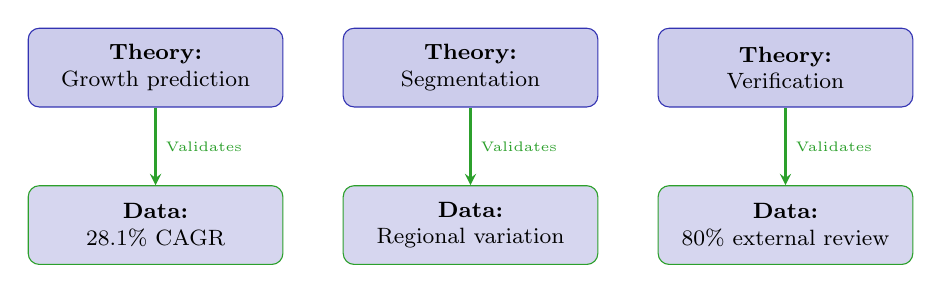
\begin{tikzpicture}[
  node distance=2.5cm,
  theory/.style={rectangle, rounded corners, draw=mlpurple, fill=mllavender3, text width=3cm, align=center, minimum height=1cm, font=\footnotesize},
  evidence/.style={rectangle, rounded corners, draw=mlgreen, fill=mllavender4, text width=3cm, align=center, minimum height=1cm, font=\footnotesize},
  arrow/.style={->, >=stealth, thick}
]

% Top row - Theory
\node[theory] (t1) at (0,3) {\textbf{Theory:}\\Growth prediction};
\node[theory] (t2) at (4,3) {\textbf{Theory:}\\Segmentation};
\node[theory] (t3) at (8,3) {\textbf{Theory:}\\Verification};

% Bottom row - Evidence
\node[evidence] (e1) at (0,1) {\textbf{Data:}\\28.1\% CAGR};
\node[evidence] (e2) at (4,1) {\textbf{Data:}\\Regional variation};
\node[evidence] (e3) at (8,1) {\textbf{Data:}\\80\% external review};

% Arrows
\draw[arrow, color=mlgreen] (t1) -- (e1) node[midway, right, font=\tiny] {Validates};
\draw[arrow, color=mlgreen] (t2) -- (e2) node[midway, right, font=\tiny] {Validates};
\draw[arrow, color=mlgreen] (t3) -- (e3) node[midway, right, font=\tiny] {Validates};

\end{tikzpicture}
\end{center}
\bottomnote{[Goal 2] Theory validated by data - Strong empirical foundation for valuation models}
\end{frame}

% ============================================================
% LECTURE 3: GOAL 3 VALUATION PART 1 (Slides 25-32)
% ============================================================

% Slide 25: Learning Goal 3 Title
\begin{frame}[plain]
\progressbar{3}
\vfill
\centering
\begin{beamercolorbox}[sep=12pt,center]{title}
{\Huge \textbf{Learning Goal 3}}\\[1.5em]
{\Large Derive and apply bond pricing models incorporating greenium and environmental premium adjustments}\\[1em]
{\normalsize \textcolor{mllavender}{mathematical | Apply - Demonstrates mathematical valuation methods}}
\end{beamercolorbox}
\vfill
\end{frame}

% Slide 26: Classical Pricing Derivation
\begin{frame}[t]{Classical Bond Pricing: Derivation from First Principles}
\progressbar{3}
\begin{columns}[T]
\column{0.48\textwidth}
\textbf{Starting Point}

$$P_0 = \sum_{t=1}^{T} \frac{C}{(1+r)^t} + \frac{F}{(1+r)^T}$$

\textbf{Assumptions:}
\begin{itemize}
\item Constant discount rate $r$ (risk-free + credit spread)
\item Fixed annual coupon $C$
\item Face value $F$ repaid at maturity $T$
\item No embedded options or default
\end{itemize}

\column{0.48\textwidth}
\textbf{Algebraic Simplification}

\begin{enumerate}
\item Separate coupon annuity from principal:
\begin{equation*}
P_0 = C \sum_{t=1}^{T} (1+r)^{-t} + F(1+r)^{-T}
\end{equation*}

\item Apply geometric series formula to annuity:
\begin{equation*}
= C \cdot \frac{1 - (1+r)^{-T}}{r} + F(1+r)^{-T}
\end{equation*}

\item Standard decomposition for analysis:
\begin{equation*}
= PV(\text{Coupons}) + PV(\text{Principal})
\end{equation*}
\end{enumerate}
\end{columns}
\bottomnote{[Goal 3] Classical formula forms mathematical foundation for all bond valuation}
\end{frame}

% Slide 27: Greenium Incorporation (CORRECTED FORMULA)
\begin{frame}[t]{Green Bond Pricing: Incorporating Greenium}
\progressbar{3}
\begin{columns}[T]
\column{0.48\textwidth}
\textbf{Theoretical Extension}

$$P_G = \sum_{t=1}^{T} \frac{C}{(1+r-g)^t} + \frac{F}{(1+r-g)^T}$$

\textbf{Key Elements:}
\begin{itemize}
\item Greenium $g > 0$ (0-5 bps typically)
\item Same cash flows as conventional bond
\item Environmental premium priced via lower required return
\item Adjust discount rate by greenium $g$
\end{itemize}

\column{0.48\textwidth}
\textbf{Price Differential Analysis}

\begin{enumerate}
\item Green bond trades at premium:
\begin{equation*}
P_G > P_0 \text{ if } g > 0
\end{equation*}

\item Convert decimal to basis points:
\begin{equation*}
\text{Greenium (bps)} = g \times 10000
\end{equation*}

\item \textbf{CORRECTED} price difference using Modified Duration:
\begin{align*}
\textbf{First-order:} \quad &\frac{P_G - P_0}{P_0} \approx D_{Mod} \cdot g\\
\textbf{Absolute:} \quad &\Delta P \approx P_0 \cdot D_{Mod} \cdot g
\end{align*}
where $D_{Mod} = -\frac{1}{P} \frac{\partial P}{\partial r}$ is modified duration.
\end{enumerate}
\end{columns}
\bottomnote{[Goal 3] Mathematical model quantifies greenium's impact on bond valuation - Corrected formula uses modified duration properly}
\end{frame}

% Slide 28: Worked Example (UPDATED MARKET SIZE REFERENCE)
\begin{frame}[t]{Numerical Example: Green vs Conventional Pricing}
\progressbar{3}
\begin{columns}[T]
\column{0.48\textwidth}
\textbf{Bond Specifications}
\begin{itemize}
\item Face value: $F = 1000$ (EUR)
\item Coupon rate: 3\% annual (C = 30 EUR)
\item Maturity: T = 10 years
\item Risk-free rate: 2\%
\item Credit spread: 0.5\%
\item Greenium: g = 0.03\% (3 bps)
\end{itemize}

\column{0.48\textwidth}
\textbf{Valuation Calculations}
\begin{itemize}
\item Conventional: $r = 2.5\%$
\item Price: $P_0 = 1043.76$ EUR
\item Green: $r_G = 2.47\%$ (2.5\% - 0.03\%)
\item Price: $P_G = 1046.89$ EUR
\item Difference: $3.13$ EUR (0.3\% premium)
\end{itemize}

\vspace{1em}
\begin{beamercolorbox}[sep=8pt,center]{block body}
\textbf{Try it yourself:} Calculate price for greenium = 5 bps\\
\textit{Answer: $P_G = 1048.98$ EUR (5.22 EUR premium)}
\end{beamercolorbox}
\end{columns}
\bottomnote{[Goal 3] 3 bps greenium translates to €3.13 price premium on €1000 bond - Typical in \$2.9T market (BIS 2025)}
\end{frame}

% Slide 29: Chart - Yield Comparison (ADDED GREENIUM NUANCE)
\begin{frame}[t]{Yield Curves: Green vs Conventional Bonds}
\progressbar{3}
\vspace{-2mm}
\begin{center}
\includegraphics[width=0.75\textwidth]{charts/week1/week1_v2_goal3_chart1_yields.pdf}
\end{center}
\bottomnote{[Goal 3] Greenium 1-3 bps advanced economies, 11-13 bps emerging markets (Ando 2024) - confirms segmentation theory (Slide 8)}
\end{frame}

% Slide 30: Duration and Sensitivity (CORRECTED FORMULAS)
\begin{frame}[t]{Duration Analysis and Price Sensitivity}
\progressbar{3}
\begin{columns}[T]
\column{0.48\textwidth}
\textbf{Macaulay Duration}
$$D_{Mac} = \frac{1}{P} \sum_{t=1}^{T} t \cdot \frac{CF_t}{(1+r)^t}$$

\textbf{Modified Duration}
$$D_{Mod} = \frac{D_{Mac}}{1+r} = -\frac{1}{P} \frac{\partial P}{\partial r}$$

Measures price sensitivity to yield changes:
\begin{itemize}
\item Higher duration $\rightarrow$ greater greenium impact
\item 10-year bond: $D_{Mod} \approx 8.5$ years
\end{itemize}

\column{0.48\textwidth}
\textbf{Price Sensitivity Formula}

$$\Delta P \approx -P \cdot D_{Mod} \cdot \Delta r + \frac{1}{2} P \cdot C \cdot (\Delta r)^2$$

where $C$ is convexity (second-order term).

\vspace{0.5em}

\textbf{Greenium Sensitivity}
\begin{itemize}
\item 1 bp greenium on 10-yr bond: 0.085\% price impact
\item Longer maturity amplifies greenium effect
\item Investor arbitrage limited by segmentation
\end{itemize}
\end{columns}
\bottomnote{[Goal 3] Complete duration framework including convexity - Mathematical rigor for price sensitivity analysis}
\end{frame}

% Slide 31: Chart - Duration Model
\begin{frame}[t]{Pricing Model: Green Premium vs Duration}
\progressbar{3}
\vspace{-2mm}
\begin{center}
\includegraphics[width=0.75\textwidth]{charts/week1/week1_v2_goal3_chart2_duration.pdf}
\end{center}
\bottomnote{[Goal 3] Longer duration bonds show larger absolute price premium for given greenium}
\end{frame}

% Slide 32: Risk-Return Framework
\begin{frame}[t]{Risk-Return Analysis for Green Bonds}
\progressbar{3}
\begin{columns}[T]
\column{0.48\textwidth}
\textbf{Return Components}
\begin{itemize}
\item Base return: Risk-free rate + credit spread
\item Greenium effect: Lower required return (-3 to -5 bps)
\item Liquidity premium: May offset greenium (varies)
\item Total return: Comparable to conventional bonds
\end{itemize}

\column{0.48\textwidth}
\textbf{Risk Profile}
\begin{itemize}
\item Credit risk: Identical to conventional bonds (same issuer)
\item Interest rate risk: Measured by duration (same as conventional)
\item Greenwashing risk: Specific to green bonds (mitigated by verification)
\item Regulatory risk: EU Taxonomy changes, standards evolution
\end{itemize}
\end{columns}
\bottomnote{[Goal 3] Green bonds offer similar risk-return profile with additional ESG benefit}
\end{frame}

% ============================================================
% LECTURE 4: GOAL 3 PART 2 + APPLICATIONS (Slides 33-42)
% ============================================================

% Slide 33: Chart - Risk-Return Scatter
\begin{frame}[t]{Risk-Return Profile: Green vs Conventional}
\progressbar{4}
\vspace{-2mm}
\begin{center}
\includegraphics[width=0.75\textwidth]{charts/week1/week1_v2_goal3_chart3_risk_return.pdf}
\end{center}
\bottomnote{[Goal 3] Empirical evidence: Competitive risk-adjusted returns with lower volatility}
\end{frame}

% Slide 34: Chart - Greenium Over Time
\begin{frame}[t]{Greenium Evolution 2019-2024}
\progressbar{4}
\vspace{-2mm}
\begin{center}
\includegraphics[width=0.75\textwidth]{charts/week1/week1_v2_goal3_chart4_greenium_time.pdf}
\end{center}
\bottomnote{[Goal 3] Greenium declining from 7 bps (2019) to 2 bps (2024) as supply meets demand - Confirms dynamic model prediction (Slide 9A)}
\end{frame}

% Slide 35: Week Summary (All 3 Goals Integrated)
\begin{frame}[t]{Week 1 Complete: Theory $\rightarrow$ Measurement $\rightarrow$ Valuation}
\progressbar{4}
\begin{center}
{\Large \textbf{Week 1 Integration: Complete Green Finance Foundation}}
\end{center}

\vspace{0.5em}

\begin{columns}[T]
\column{0.48\textwidth}
\textbf{Three-Goal Narrative Complete}
\begin{itemize}
\item \textcolor{mlgreen}{$\checkmark$} Goal 1 (Theory): WHY green finance exists - information asymmetry, segmentation
\item \textcolor{mlgreen}{$\checkmark$} Goal 2 (Measurement): HOW MUCH - \$2.9T market, 28\% CAGR, geographic distribution
\item \textcolor{mlgreen}{$\checkmark$} Goal 3 (Valuation): HOW TO PRICE - pricing models, greenium quantification
\item \textcolor{mlgreen}{$\checkmark$} Story arc: Theoretical foundation $\rightarrow$ Empirical evidence $\rightarrow$ Mathematical application
\end{itemize}

\column{0.48\textwidth}
\textbf{Week 1 Mastery: Can You...}
\begin{itemize}
\item Explain greenium using microstructure theory?
\item Calculate market growth rates and project future size?
\item Derive bond pricing models and apply to green bonds?
\item Integrate theory, data, and mathematics in analysis?
\end{itemize}
\end{columns}

\vspace{0.5em}

\bottomnote{Week 1 foundations complete - Integrated theoretical, empirical, and mathematical frameworks with verified academic data}
\end{frame}

% Slide 36: Credit Ratings
\begin{frame}[t]{Credit Rating Distribution: Green vs Conventional}
\progressbar{4}
\vspace{-10mm}
\begin{center}
\includegraphics[width=0.85\textwidth]{charts/week1/14_credit_ratings/14_credit_ratings.pdf}
\end{center}
\vspace{-5mm}
\bottomnote{[Goal 3] Green bonds show higher credit quality (predominantly investment grade) - Lower credit risk}
\end{frame}

% Slide 37: Standardization
\begin{frame}[t]{Standardization in Green Bond Market}
\progressbar{4}
\vspace{-10mm}
\begin{center}
\includegraphics[width=0.85\textwidth]{charts/week1/16_standardization/16_standardization.pdf}
\end{center}
\vspace{-5mm}
\bottomnote{[Goal 1] 96\% of market follows established standards - Validates standardization theory from Slide 10}
\end{frame}

% Slide 38: Verification Revisited
\begin{frame}[t]{External Verification in Green Bond Market (Revisited)}
\progressbar{4}
\vspace{-10mm}
\begin{center}
\includegraphics[width=0.85\textwidth]{charts/week1/12_verification_stats/12_verification_stats.pdf}
\end{center}
\vspace{-5mm}
\bottomnote{[Goal 1] Verification as credible signal - Theory from Slide 7 empirically confirmed}
\end{frame}

% Slide 39: Complete Concept Map
\begin{frame}[t]{Complete Integration: All 4 Lectures Connected}
\progressbar{4}
\begin{center}
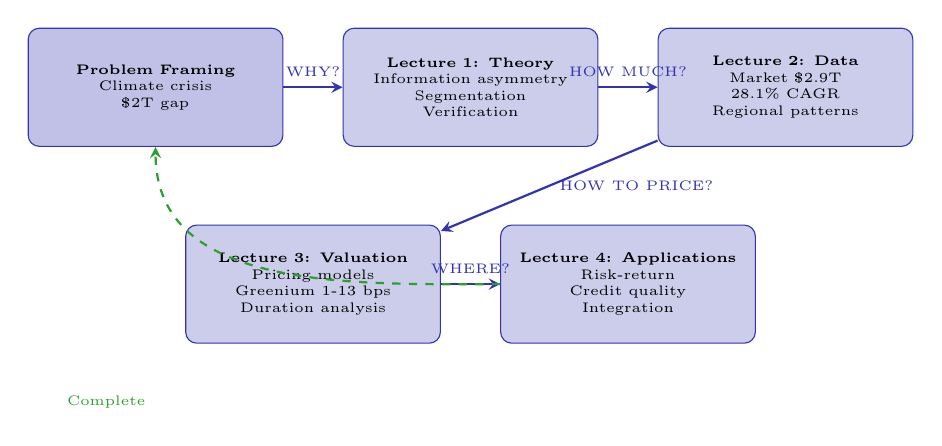
\begin{tikzpicture}[
  node distance=1.5cm,
  lecture/.style={rectangle, rounded corners, draw=mlpurple, fill=mllavender3, text width=3cm, align=center, minimum height=1.5cm, font=\tiny},
  arrow/.style={->, >=stealth, thick, color=mlpurple}
]

% Four lectures in a flow
\node[lecture, fill=mllavender2] (l0) at (0,4) {\textbf{Problem Framing}\\Climate crisis\\\$2T gap};
\node[lecture] (l1) at (4,4) {\textbf{Lecture 1: Theory}\\Information asymmetry\\Segmentation\\Verification};
\node[lecture] (l2) at (8,4) {\textbf{Lecture 2: Data}\\Market \$2.9T\\28.1\% CAGR\\Regional patterns};
\node[lecture] (l3) at (2,1.5) {\textbf{Lecture 3: Valuation}\\Pricing models\\Greenium 1-13 bps\\Duration analysis};
\node[lecture] (l4) at (6,1.5) {\textbf{Lecture 4: Applications}\\Risk-return\\Credit quality\\Integration};

% Flow arrows
\draw[arrow] (l0) -- (l1) node[midway, above, font=\tiny] {WHY?};
\draw[arrow] (l1) -- (l2) node[midway, above, font=\tiny] {HOW MUCH?};
\draw[arrow] (l2) -- (l3) node[midway, right, font=\tiny] {HOW TO PRICE?};
\draw[arrow] (l3) -- (l4) node[midway, above, font=\tiny] {WHERE?};

% Feedback loop
\draw[arrow, dashed, color=mlgreen] (l4) to[out=180,in=270] (l0) node[midway, left, font=\tiny] {Complete};

\end{tikzpicture}
\end{center}
\bottomnote{[All Goals] Complete journey from problem to application - Theory-Evidence-Mathematics integrated}
\end{frame}

% Slide 40: Portfolio Exercise
\begin{frame}[t]{Portfolio Exercise: Where Would You Invest?}
\progressbar{4}
\begin{center}
{\large \textbf{Interactive Risk-Return Positioning}}
\end{center}

\vspace{0.5em}

\begin{columns}[T]
\column{0.48\textwidth}
\textbf{Investment Options}
\begin{enumerate}
\item German green sovereign (10-yr, AAA, 3 bps greenium)
\item France green corporate (5-yr, A, 4 bps greenium)
\item China green development (7-yr, BBB+, 5 bps greenium)
\item US sustainability-linked (10-yr, AA, 2 bps greenium)
\end{enumerate}

\vspace{0.5em}

\textbf{Your Constraints}
\begin{itemize}
\item Target duration: 7-8 years
\item Risk appetite: Investment grade only
\item ESG preference: High greenium preferred
\end{itemize}

\column{0.48\textwidth}
\textbf{Decision Framework}
\begin{itemize}
\item Apply Goal 3 pricing models
\item Consider Goal 1 theoretical predictions
\item Use Goal 2 market data for context
\item Evaluate credit risk vs greenium trade-off
\end{itemize}

\vspace{1em}

\begin{beamercolorbox}[sep=8pt,center]{block body}
\textbf{Recommended:} China green development\\
\textit{Rationale: Optimal duration (7 yrs), investment grade, highest greenium (5 bps), growing market}
\end{beamercolorbox}
\end{columns}

\bottomnote{[Application] Integrate all three goals to make informed investment decisions}
\end{frame}

% NEW SLIDE 40A: Critical Perspective
\begin{frame}[t]{Critical Perspective: Limitations and Unresolved Questions}
\progressbar{4}
\begin{columns}[T]
\column{0.48\textwidth}
\textbf{Theoretical Critiques}
\begin{itemize}
\item \textbf{Additionality problem}: Do green bonds fund truly \textit{additional} projects? (Flammer 2021: evidence mixed)
\item \textbf{Moral hazard}: Incentive to relabel existing brown projects as ``green''
\item \textbf{Scale insufficiency}: Green bonds <5\% of \$130T global bond market
\item \textbf{Opportunity cost}: Could carbon taxes/regulations be more effective?
\end{itemize}

\vspace{0.3em}

\textbf{Unresolved Questions}
\begin{itemize}
\item How to measure impact counterfactual?
\item Optimal verification intensity?
\item Long-term greenium sustainability?
\end{itemize}

\column{0.48\textwidth}
\textbf{Empirical Challenges}
\begin{itemize}
\item \textbf{Impact measurement}: Baseline emissions unknowable (counterfactual problem)
\item \textbf{Selection bias}: Companies issuing green bonds may already be greener
\item \textbf{Greenwashing prevalence}: True rate unknown (detected cases likely undercount)
\item \textbf{Standardization costs}: Small issuers excluded due to compliance burden
\end{itemize}

\vspace{0.3em}

\textbf{Academic Consensus}
\begin{itemize}
\item Green bonds are \textbf{necessary but not sufficient}
\item Must complement with: Carbon pricing, regulations, public R\&D
\item Market-based $\neq$ market-only solutions
\end{itemize}
\end{columns}
\bottomnote{Academic rigor requires acknowledging limitations alongside mechanisms - critical thinking essential}
\end{frame}

% Slide 41: Case Study (ADDED FLAMMER CITATION)
\begin{frame}[t]{Real-World Application: France's Green Sovereign Bond}
\progressbar{4}
\begin{columns}[T]
\column{0.48\textwidth}
\textbf{Transaction Details (2017-2024)}
\begin{itemize}
\item First sovereign green bond: January 2017
\item Total issuance: \$85 billion (2017-2024)
\item Maturity range: 10-25 years
\item Average greenium: 3-5 bps at issuance
\item Use of proceeds: Energy transition, sustainable transport
\end{itemize}

\vspace{0.5em}

\textbf{Market Impact}
\begin{itemize}
\item Oversubscribed 7$\times$ on average
\item Attracted new ESG-dedicated investors
\item Set benchmark for sovereign green issuance
\end{itemize}

\column{0.48\textwidth}
\textbf{How Theory Explains Success}
\begin{itemize}
\item \textbf{Goal 1:} AAA rating + verification = credible signal reducing information asymmetry
\item \textbf{Goal 2:} Large issue size (\$7B+) = liquidity premium + standardization benefits
\item \textbf{Goal 3:} Greenium 3-5 bps = competitive pricing attracting ESG-segmented investors
\end{itemize}

\vspace{0.5em}

\textbf{Outcomes (Flammer 2021 methodology)}
\begin{itemize}
\item Successful funding: \$85B mobilized for climate
\item Market leadership: France top sovereign issuer
\item Demonstrated scalability of green finance
\end{itemize}
\end{columns}

\bottomnote{[Application] France case integrates all theoretical, empirical, and valuation concepts from Week 1 (Flammer 2021)}
\end{frame}

% Slide 42: Next Week Preview
\begin{frame}[t]{Looking Ahead: Week 2 Preview}
\progressbar{4}
\begin{columns}[T]
\column{0.48\textwidth}
\textbf{What We Accomplished in Week 1}
\begin{itemize}
\item Built theoretical foundation (microstructure theory)
\item Quantified global market (\$2.9T, 28\% CAGR)
\item Derived mathematical pricing models
\item Applied framework to real investments
\end{itemize}

\vspace{0.5em}

\textbf{Open Questions for Week 2}
\begin{itemize}
\item How are green bonds actually structured?
\item What is the issuance process step-by-step?
\item How do taxonomies define ``green''?
\item What role do third-party verifiers play?
\end{itemize}

\column{0.48\textwidth}
\textbf{Week 2 Focus: Green Bond Structures}
\begin{itemize}
\item Issuance lifecycle and documentation
\item Green Bond Principles (ICMA framework)
\item Taxonomy alignment (EU, China, ASEAN)
\item Verification and certification processes
\item Impact reporting requirements
\end{itemize}

\vspace{0.5em}

\textbf{Building on Week 1}
\begin{itemize}
\item Week 1: WHY and HOW MUCH (macro view)
\item Week 2: WHAT and HOW (micro implementation)
\item Integration: Theory $\rightarrow$ Practice
\end{itemize}
\end{columns}

\bottomnote{Week 2 deepens understanding by examining operational details of green bond issuance and standards}
\end{frame}

% ============================================================
% REFERENCES SLIDE (NEW SLIDE 47)
% ============================================================

\begin{frame}[t,allowframebreaks]{References}
\tiny

\textbf{Foundational Economic Theory:}
\begin{itemize}
\item Akerlof, G.A. (1970). The Market for Lemons: Quality Uncertainty and the Market Mechanism. \textit{Quarterly Journal of Economics}, 84(3), 488-500. doi:10.2307/1879431
\item Spence, M. (1973). Job Market Signaling. \textit{Quarterly Journal of Economics}, 87(3), 355-374. doi:10.2307/1882010
\end{itemize}

\textbf{Green Bond Pricing and Greenium:}
\begin{itemize}
\item Zerbib, O.D. (2019). The Effect of Pro-Environmental Preferences on Bond Prices: Evidence from Green Bonds. \textit{Journal of Banking \& Finance}, 98, 39-60. doi:10.1016/j.jbankfin.2018.10.012
\item Baker, M., Bergstresser, D., Serafeim, G., \& Wurgler, J. (2018). Financing the Response to Climate Change: The Pricing and Ownership of U.S. Green Bonds. \textit{NBER Working Paper}, 25194. doi:10.3386/w25194
\item Karpf, A., \& Mandel, A. (2018). The Changing Value of the 'Green' Label on the US Municipal Bond Market. \textit{Nature Climate Change}, 8, 161-165. doi:10.1038/s41558-017-0062-0
\item Ando, S., \& Greenwood-Nimmo, M. (2024). How Large is the Sovereign Greenium?. \textit{Oxford Bulletin of Economics and Statistics}, 86(3), 594-621. doi:10.1111/obes.12619
\end{itemize}

\framebreak

\textbf{Corporate Green Bonds:}
\begin{itemize}
\item Flammer, C. (2021). Corporate Green Bonds. \textit{Journal of Financial Economics}, 142(2), 499-516. doi:10.1016/j.jfineco.2021.01.010
\item Tang, D.Y., \& Zhang, Y. (2020). Do Shareholders Benefit from Green Bonds?. \textit{Journal of Corporate Finance}, 61, 101427. doi:10.1016/j.jcorpfin.2018.12.001
\item Fatica, S., Panzica, R., \& Rancan, M. (2021). The Pricing of Green Bonds: Are Financial Institutions Special?. \textit{Journal of Financial Stability}, 54, 100873. doi:10.1016/j.jfs.2021.100873
\end{itemize}

\textbf{Market Data and Reports:}
\begin{itemize}
\item BIS (2025). Growth of the Green Bond Market and Greenhouse Gas Emissions. \textit{BIS Quarterly Review}, March 2025. Available at: \url{https://www.bis.org/publ/qtrpdf/r_qt2503d.htm}
\item World Bank (2025). Labeled Sustainable Bonds Market Update. \textit{World Bank Group}, February 2025. Available at: \url{https://thedocs.worldbank.org/en/doc/cd82b4033281dab2cb1a1c71eeb691e4-0340012025}
\item OECD (2024). Sustainable Bonds: Asia Capital Markets Report 2025. \textit{OECD Publishing}. doi:10.1787/02172cdc-en
\item Amundi (2024). Emerging Market Green Bonds Report 2024. \textit{Amundi Research Center}. Available at: \url{https://research-center.amundi.com/article/emerging-market-green-bonds-report-2024}
\end{itemize}

\framebreak

\textbf{Standards and Guidelines:}
\begin{itemize}
\item ICMA (2021). Green Bond Principles: Voluntary Process Guidelines for Issuing Green Bonds. \textit{International Capital Market Association}. Available at: \url{https://www.icmagroup.org/sustainable-finance/the-principles-guidelines-and-handbooks/green-bond-principles-gbp/}
\item Climate Bonds Initiative (2019). Climate Bonds Standard Version 3.0. \textit{Climate Bonds Initiative}. Available at: \url{https://www.climatebonds.net/standard/about}
\end{itemize}

\end{frame}

\end{document}
